\chapter{Methods and Prototype}

In this section, the used methods are laid out and the implemented prototype is described. 
\section{Methods used}
\subsection{MapReduce}
At the very core of this thesis lies the idea of MapReduce, a programming model made popular by Google and presented in \cite{Dean2008}. Having large data sets to analyse that may not be handled by only few computers, like the millions of Websites gathered by Google each day that have to be indexed fast and reliably, MapReduce  provides a way of automatic parallelisation and distribution of large-scale computations. Users only need to define two types of functions: a map and a reduce function. Each computation expressed by these functions takes a set of input key/value pairs and produces a set of output key/value pairs.
A map function takes an input pair and produces a set of \textit{intermediate} key/value pairs. Once the intermediate values for each intermediate key \textit{I} are grouped together, they are passed to the reduce function. 
The reduce function then takes an intermediate key \textit{I} and the corresponding set of intermediate values (usually supplied as an iterator to the reduce function) and merges them according to user-specified code into a possibly smaller set of values. The resulting key and value are then written to an output file, allowing to handle lists of values that are too large to fit in memory. 

A very simple yet often used MapReduce operation is to count words in a collection of documents, the so called \textit{WordCount}. Below pseudocode demonstrates how one can count all the words in documents using map and reduce functions.

\begin{algorithmic}
\Function{map}{String key, String value}
\State \textit{// key: document name, value: document content}

\For{word $w$ in values}
\State EmitIntermediate($w$, $"1"$);
\EndFor
\EndFunction


\Function{reduce}{String key, Iterator values}
\State \textit{// key: a word, values: a list of "1"'s}
\State int $result$ = 0;
\For{$v$ in values}
\State $result$ += ParseInt($v$);
\EndFor
\State Emit(AsString($result$));
\EndFunction
\end{algorithmic}

The map function splits the received text (\textit{value}) into all corresponding words and for each word, emits its occurrence count (simply a 1). The reduce function then takes, for each word individually (\textit{key}), these occurrences (\textit{values}) and sums them up, eventually emitting for each word the sum of occurrences (\textit{result}). Although above pseudocode suggests inputs and outputs to be strings, the user specifies the associated types. This means that input keys and values may be of a different domain than the output keys and values (note that the \textit{intermediate} keys and values are from the same domain as the output keys and values). Conceptually, this is expressed as follows:
\newline
\newline
\begin{tabular}{lll}
map	& (k1, v1) & $\to$ list(k2, v2)\\
reduce & (k2, list(v2)) & $\to$ list(v2)
\end{tabular}

The traditional way to view the workflow in a MapReduce program is indicated by Figure \ref{fig:mapreduce_workflow}. A master schedules execution and assigns tasks to workers, which then perform the actual map or reduce on the assigned data. Input data is partitioned into \textit{M} splits with a size of around 16-64 MB per piece to be processed in parallel by different machines, and the intermediate key space is partitioned into \textit{R} pieces, where R usually is the number of available workers for executing reduce but may also be specified by the user. To evenly distribute these pieces, a partitioning function like \textit{hash(key) mod R} may be used. In such a setting, same intermediate keys may not be grouped together, which is done before the reduce action is performed. Additional combination in between may be applied to reduce the amount of data to be distributed among the workers.

\begin{figure}
	\centering	
	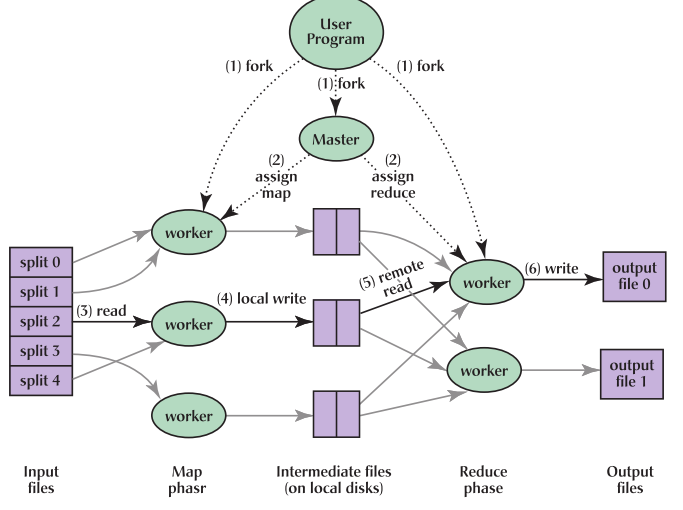
\includegraphics{mapreduce_workflow}
	\caption{Execution overview in a typical MapReduce program}	
	\label{fig:mapreduce_workflow}
\end{figure} 
\section{Prototype}
